\section[cnn]{Convolutional Networks / Representation Learning}

\begin{frame}
  \frametitle{Image classification}
    \begin{center}
      \begin{tikzpicture}
        \node[anchor=north west,inner sep=0] (image) at (1,-1) {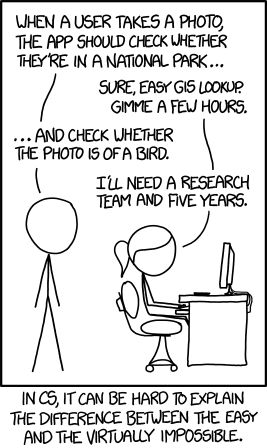
\includegraphics[width=0.3\textwidth]{xkcd.png}};
        \node[anchor=north west,inner sep=0] at (image.south west)  {\small{\url{http://xkcd.com/1425/}}};
        \node[anchor=north west,inner sep=0] at (5,-3) {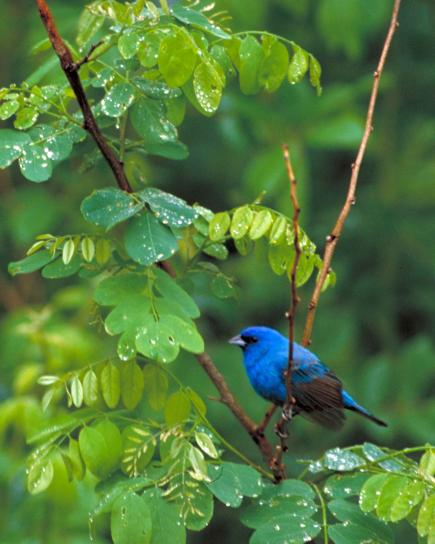
\includegraphics[width=0.3\textwidth]{bird5.png}};
        \node[anchor=north west,inner sep=0] at (-3,0) {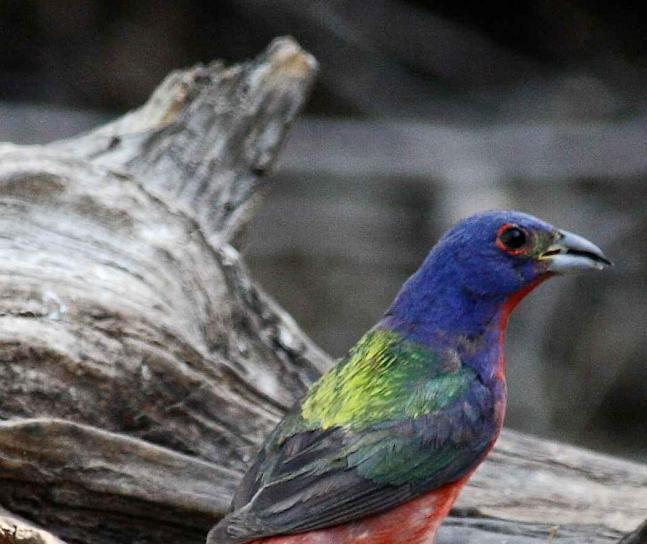
\includegraphics[width=0.3\textwidth]{bird1.png}};
        \node[anchor=north west,inner sep=0] at (-3,-2.5) {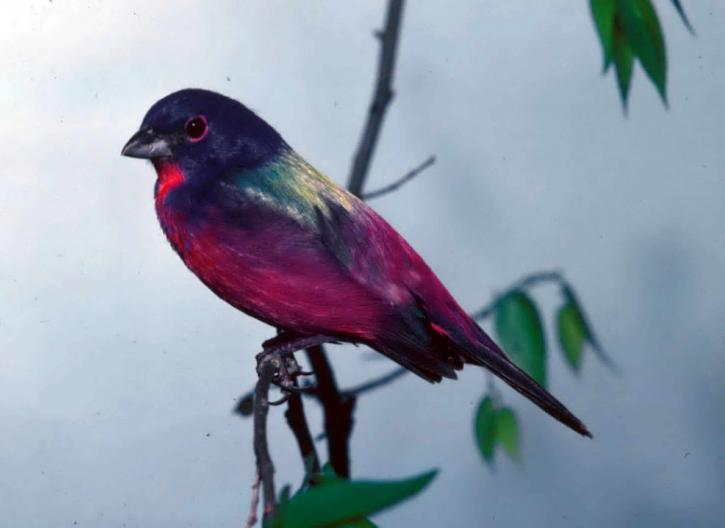
\includegraphics[width=0.3\textwidth]{bird2.png}};
        \node[anchor=north west,inner sep=0] at (-3,-5) {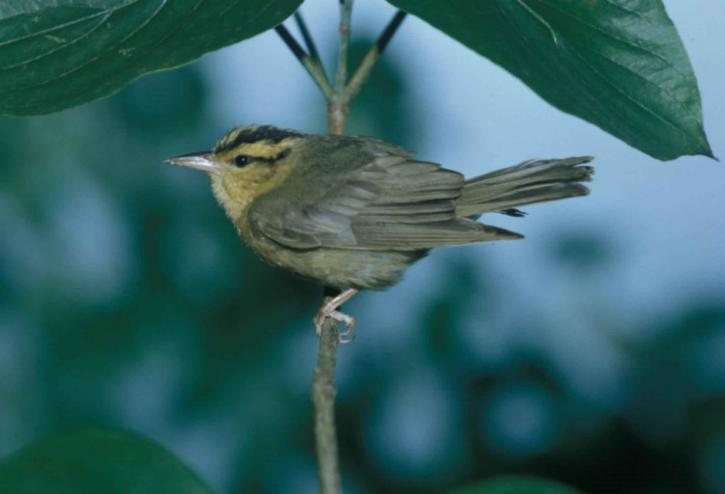
\includegraphics[width=0.3\textwidth]{bird3.png}};
        \node[anchor=north west,inner sep=0] at (5,0) {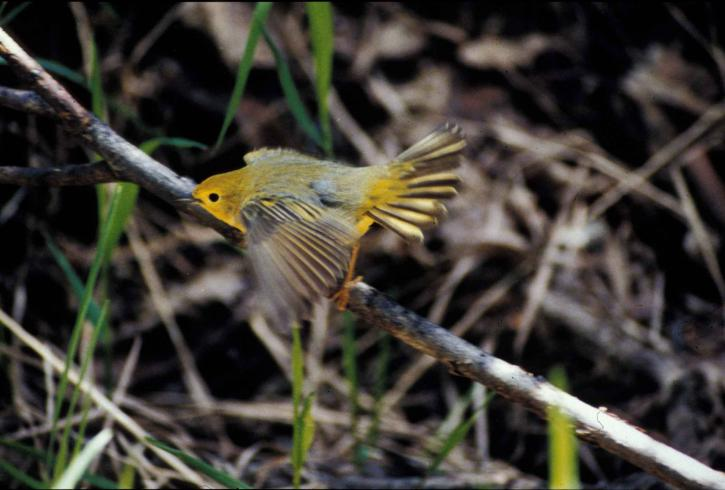
\includegraphics[width=0.3\textwidth]{bird4.png}};
        \node[anchor=north west,inner sep=0] at (5,-2) {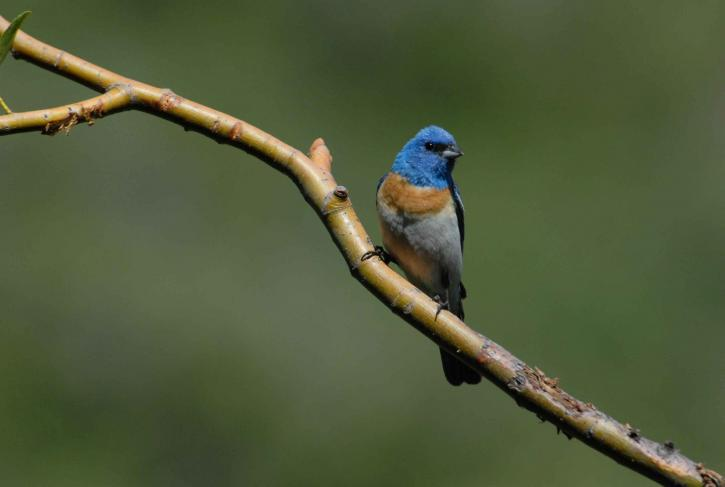
\includegraphics[width=0.3\textwidth]{bird6.png}};
      \end{tikzpicture}

      Lots of different birds in different poses, scales and positions!
    \end{center}
\end{frame}


\begin{frame}
  \frametitle{Invariance under Transformations}
    \begin{center}
      \textbf{Different strategies to build a classifier which is invariant under given transformations in the input space}:
      \begin{itemize}
        \item Extract hand-crafted features that are invariant
        \item Use transformed copies during the training phase
        \item Penalize change in the output under input transformation $\rightarrow$ Tangent propagation
        \item \textbf{Build invariance properties into structure of neural network}
      \end{itemize}
      \begin{tikzpicture}
        \node[anchor=north west,inner sep=0] at (0,0) {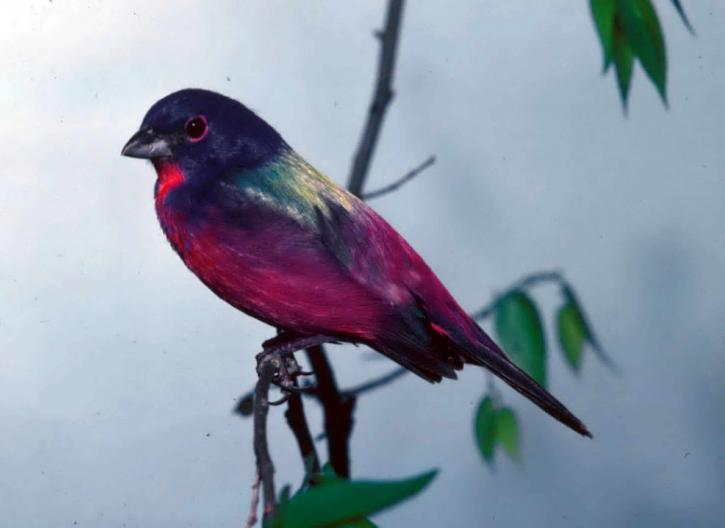
\includegraphics[width=0.21\textwidth]{bird2.png}};
        \node[anchor=north west,inner sep=0] at (2.5,0) {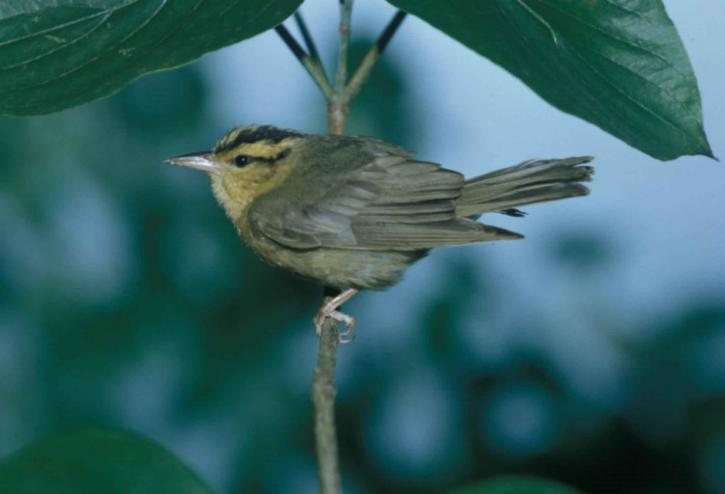
\includegraphics[width=0.23\textwidth]{bird3.png}};
        \node[anchor=north west,inner sep=0] at (5,0) {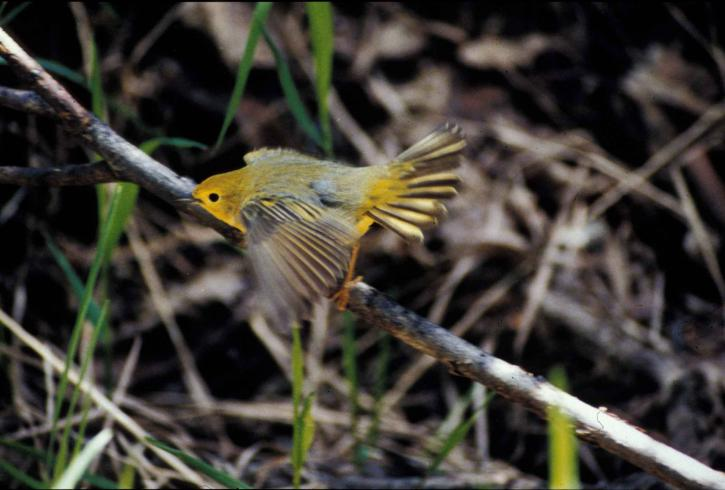
\includegraphics[width=0.23\textwidth]{bird4.png}};
        \node[anchor=north west,inner sep=0] at (7.5,0) {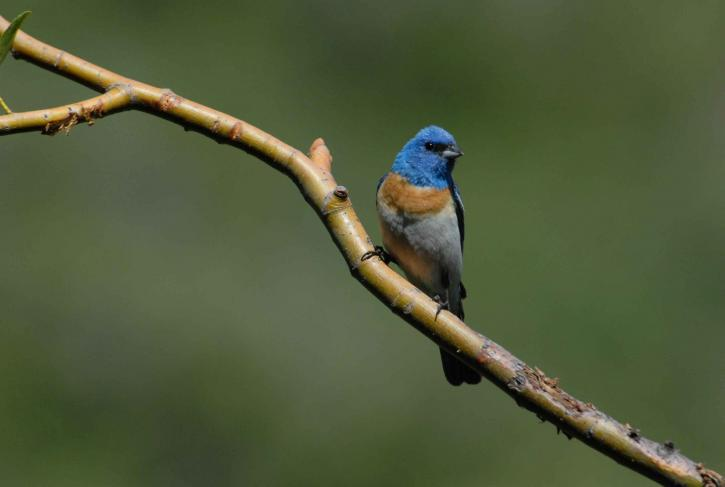
\includegraphics[width=0.23\textwidth]{bird6.png}};
      \end{tikzpicture}
    \end{center}
\end{frame}

\begin{frame}
  \frametitle{Key Idea}
    \begin{center}
      \begin{tikzpicture}[scale=0.5]

        \draw[line width=0.05cm,->] (-6,6) -> (-6,-4) node[midway,sloped,above,rotate=180] {Increasing Abstraction};
        \draw[line width=0.05cm,->] (7,6) -> (7,-4) node[midway,sloped,above] {Increasing Invariance};
        
        \node[anchor=center] at (0.5, 7.5) {Pixels from Image};
        \draw (-4,6) -- (0.5,7);
        \draw (-1,6) -- (0.5,7);
        \draw (2,6) -- (0.5,7);
        \draw (5,6) -- (0.5,7);

        \begin{scope}
          \clip (-4,5) circle (1cm);
          \draw[line width=0.05cm] (-4,5) circle (1cm);
          \draw[line width=0.1cm] (-6,5) -- (-3,5);
        \end{scope}

        \begin{scope}
          \clip (-1,5) circle (1cm);
          \draw[line width=0.05cm] (-1,5) circle (1cm);
          \draw[line width=0.1cm] (-0.4,4.4) arc (0:110:1cm);
        \end{scope}

        \begin{scope}
          \clip (2,5) circle (1cm);
          \draw[line width=0.05cm] (2,5) circle (1cm);
          \draw[line width=0.1cm] (2,5) circle (0.5cm);
        \end{scope}

        \begin{scope}
          \clip (5,5) circle (1cm);
          \draw[line width=0.05cm] (5,5) circle (1cm);
          \draw[line width=0.1cm] (4.5,5.5) -- (5.5,5.5) -- (5.5,4.5);
        \end{scope}

        \begin{scope}
          \clip (-4,1) circle (1cm);
          \draw[line width=0.05cm] (-4,1) circle (1cm);
          \shade[inner color=black,outer color=yellow] (-4,1) circle (1cm);
        \end{scope}

        \begin{scope}
          \clip (-1,1) circle (1cm);
          \draw[line width=0.05cm] (-1,1) circle (1cm);
          \shade[left color=black,right color=white!80!black] (-1.5,1.8) -- (-0.5,1.8) -- (-1.0,0.2) -- cycle;
        \end{scope}

        \draw (-4,5-1) -- (-4,1+1);
        \draw (-4,5-1) -- (-1,1+1);
        \draw (-4,5-1) -- (2,1+1);
        \draw (-4,5-1) -- (5,1+1);
        
        \draw (-1,5-1) -- (-4,1+1);
        \draw (-1,5-1) -- (-1,1+1);
        \draw (-1,5-1) -- (2,1+1);
        \draw (-1,5-1) -- (5,1+1);
        \draw (2,5-1) -- (-4,1+1);
        \draw (2,5-1) -- (-1,1+1);
        \draw (2,5-1) -- (2,1+1);
        \draw (2,5-1) -- (5,1+1);
        
        \draw (5,5-1) -- (-4,1+1);
        \draw (5,5-1) -- (-1,1+1);
        \draw (5,5-1) -- (2,1+1);
        \draw (5,5-1) -- (5,1+1);
        
        
        \draw (-4,1-1) -- (-4,-3+1);
        \draw (-4,1-1) -- (-1,-3+1);
        \draw (-4,1-1) -- (2,-3+1);
        \draw (-4,1-1) -- (5,-3+1);
        
        \draw (-1,1-1) -- (-4,-3+1);
        \draw (-1,1-1) -- (-1,-3+1);
        \draw (-1,1-1) -- (2,-3+1);
        \draw (-1,1-1) -- (5,-3+1);
        
        \draw (2,1-1) -- (-4,-3+1);
        \draw (2,1-1) -- (-1,-3+1);
        \draw (2,1-1) -- (2,-3+1);
        \draw (2,1-1) -- (5,-3+1);
        
        \draw (5,1-1) -- (-4,-3+1);
        \draw (5,1-1) -- (-1,-3+1);
        \draw (5,1-1) -- (2,-3+1);
        \draw (5,1-1) -- (5,-3+1);
        
        \begin{scope}
          \clip (2,1) circle (1cm);
          \draw[line width=0.05cm] (2,1) circle (1cm);
          \draw[line width=0.1cm] (2,2) -- (2,1);
          \draw[line width=0.1cm] (2,1) -- (2.8,0.3);
          \draw[line width=0.1cm] (2,1) -- (2,0.0);
          \draw[line width=0.1cm] (2,1) -- (1.2,0.3);
        \end{scope}
        
        \begin{scope}
          \clip (5,1) circle (1cm);
          \draw[line width=0.05cm] (5,1) circle (1cm);
          \shade[top color=black, bottom color=brown] (5,1) circle (1cm and 0.6cm);
        \end{scope}

        \begin{scope}
        \clip (-4,-3) circle (1cm);
        \node[anchor=center,inner sep=0] at (-4,-3) {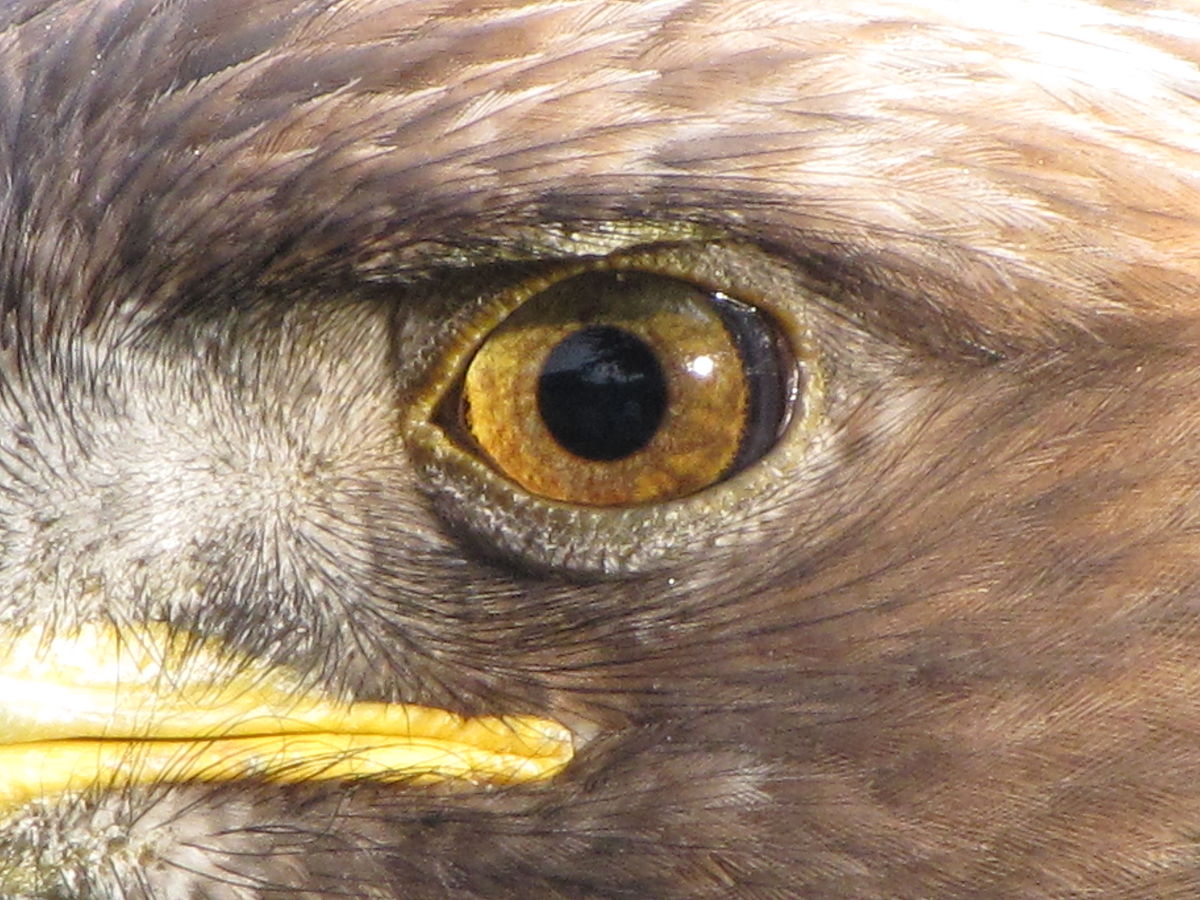
\includegraphics[height=0.2\textheight]{bird_eye.jpg}};
        \end{scope}        
        \begin{scope}
        \clip (-1,-3) circle (1cm);
        \node[anchor=center,inner sep=0] at (-1,-3) { 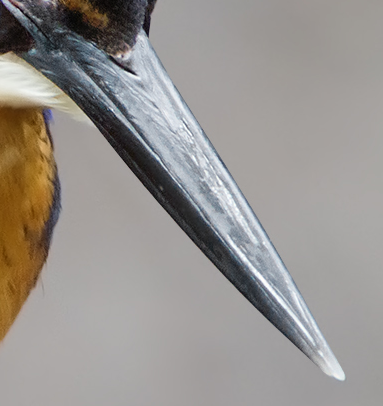
\includegraphics[height=0.15\textheight]{bird_bleak.png}};
        \end{scope}
        \begin{scope}
        \clip (2,-3) circle (1cm);
        \node[anchor=center,inner sep=0] at (2,-3) {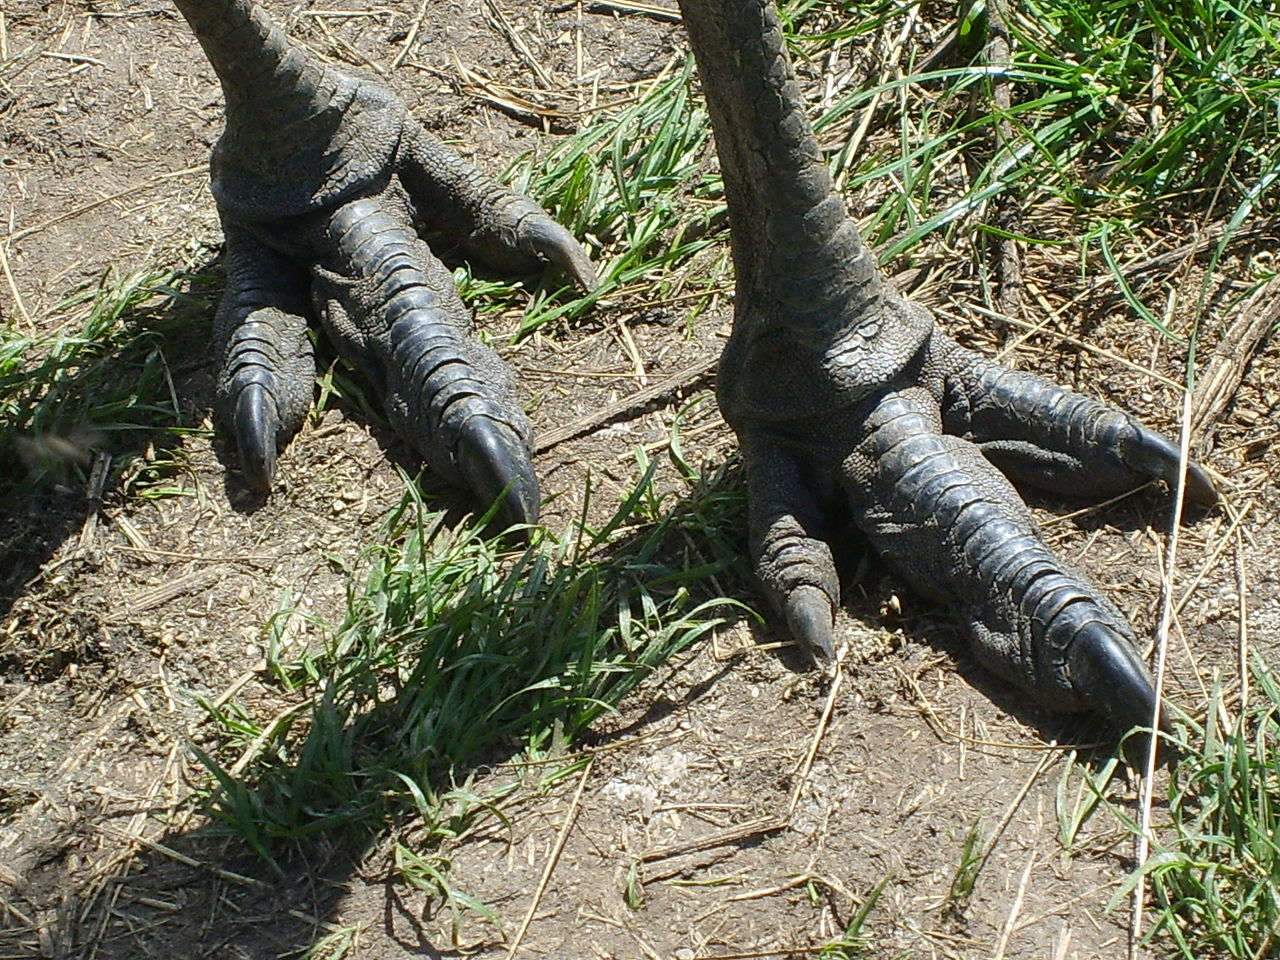
\includegraphics[height=0.1\textheight]{bird_foot.jpg}};
        \end{scope}
        \begin{scope}
        \clip (5,-3) circle (1cm);
          \node[anchor=center,inner sep=0]  at (5, -3) {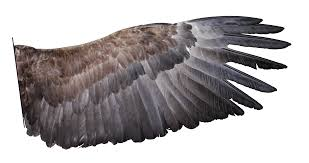
\includegraphics[height=0.1\textheight]{bird_wing.jpeg}};
        \end{scope}
        
        \draw (-4,-3-1) -- (0.5,-5);
        \draw (-1,-3-1) -- (0.5,-5);
        \draw (2,-3-1) -- (0.5,-5);
        \draw (5,-3-1) -- (0.5,-5);
        \node[anchor=center] at (0.5, -5.5) {Classification: Bird};
      \end{tikzpicture}

    \end{center}
\end{frame}


\begin{frame}
  \frametitle{Park or Bird?}
    \begin{center}
      \begin{tikzpicture}
        \node[anchor=north west,inner sep=0] (image) at (0,0) {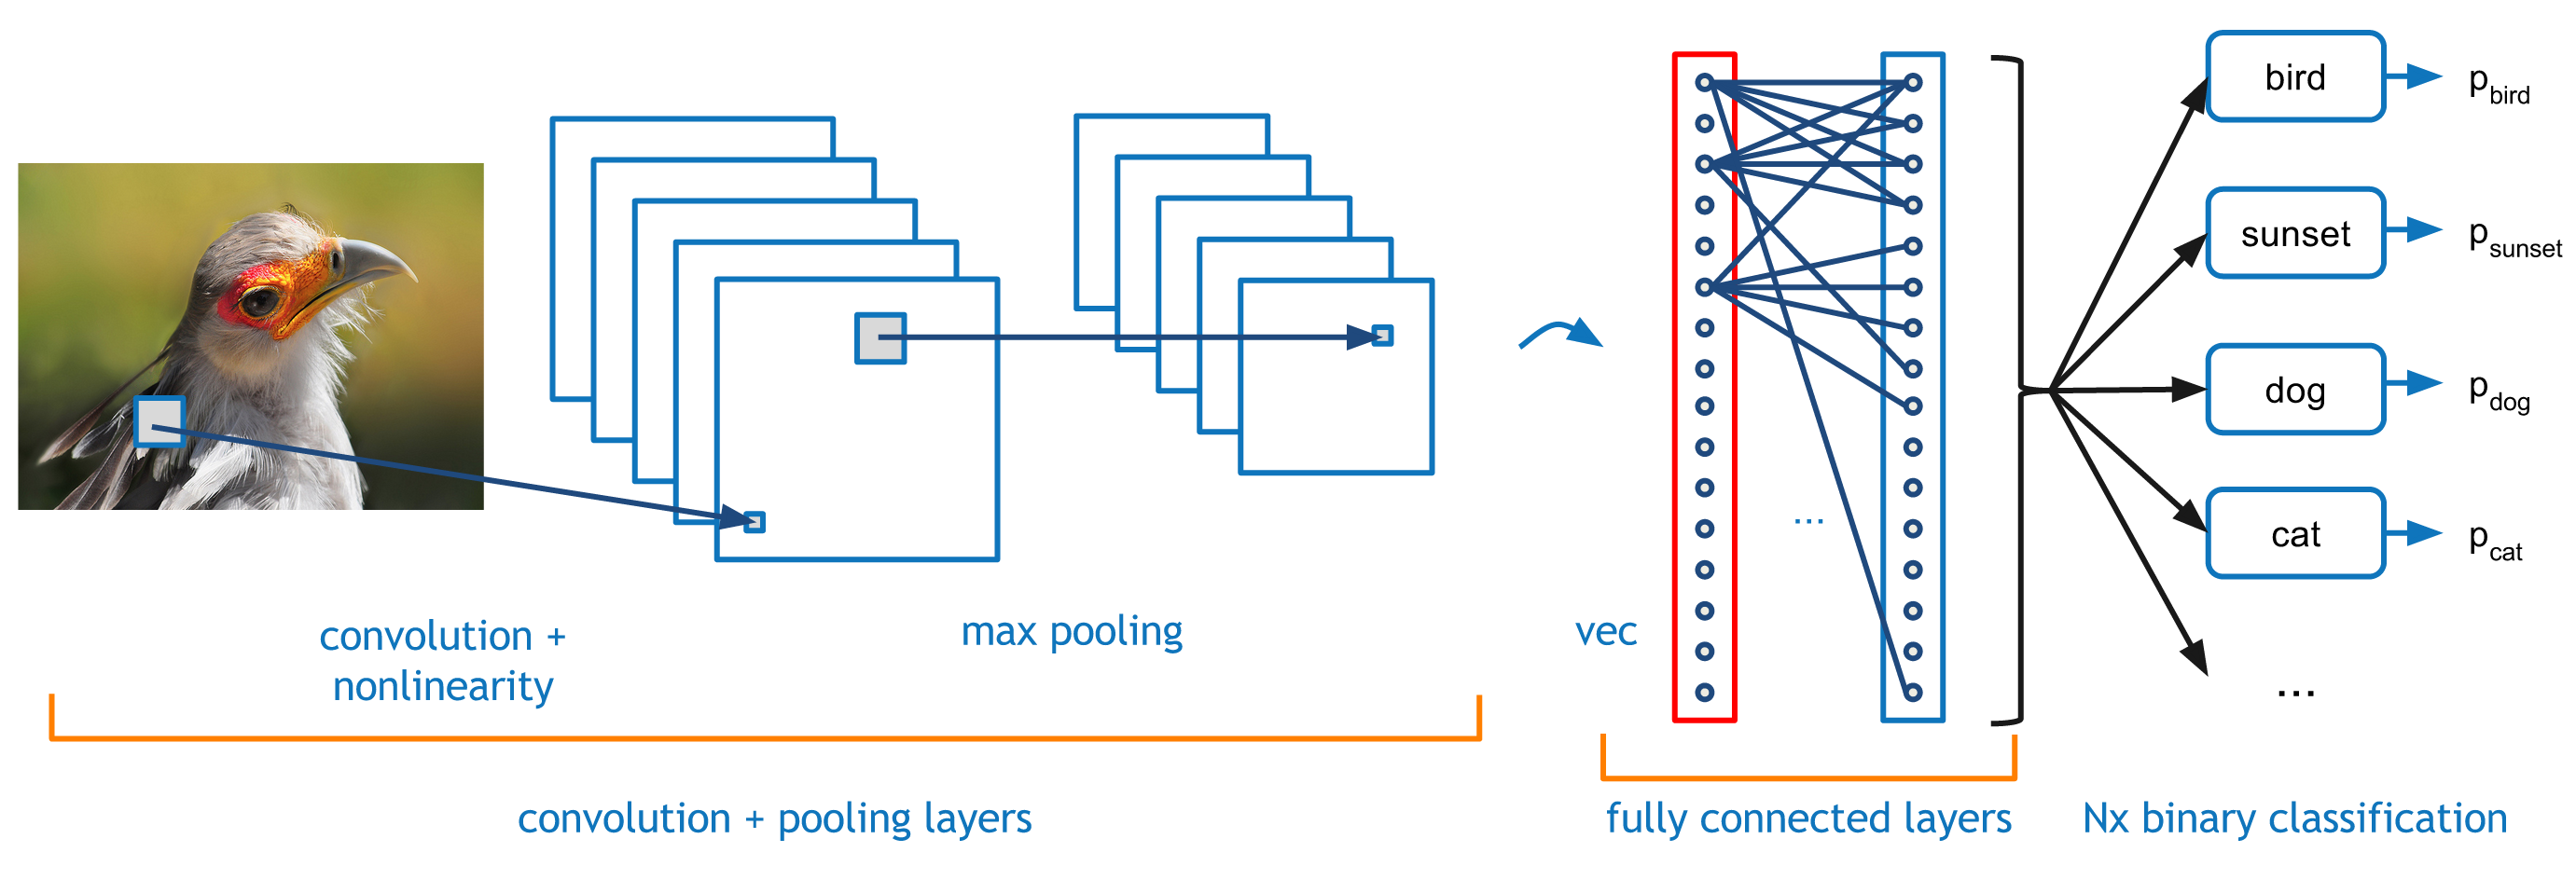
\includegraphics[width=\textwidth]{conv-net2.png}};
        \node[anchor=north west,inner sep=0] at (image.south west) {\url{http://parkorbird.flickr.com/}};
      \end{tikzpicture}
        \textbf{Convolutional layer}
        \begin{itemize}
          \item Learnable filters (e.g. edge detector) organized in feature maps
          \item Each filter scans the image and detects a specific pattern
        \end{itemize}
    \end{center}
\end{frame}

\begin{frame}[fragile]
\frametitle{Details: Convolutional Layer}
\begin{center}
      \begin{tikzpicture}
      \draw[step=0.5cm,color=gray] (-2,-2) grid (2,2);
      \matrix[matrix of nodes,nodes={inner sep=0pt,text width=.5cm,align=center,minimum height=.5cm, color=gray}]{
      78 & 89 & 29 & 84 & 71 & 33 & 31 & 86 \\
      79 & 27 & 35 & 35 & 94 & 61 & 36 & 19 \\
      22 & 17 & 7 & 45 & 30 & 40 & 29 & 72 \\
      35 & 14 & 11 & 37 & 66 & 76 & 3 & 88 \\
      59 & 4 & 11 & 13 & 22 & 57 & 10 & 52 \\
      62 & 95 & 52 & 19 & 58 & 59 & 22 & 10\\
      9 & 10 & 24 & 42 & 8 & 11 & 87 & 50 \\
      92 & 39 & 53 & 90 & 62 & 78 & 33 & 41\\
       };
     
        \matrix[matrix of nodes,nodes={inner sep=0pt,text width=.5cm,align=center,minimum height=.5cm,fill=red,fill opacity=0.8,draw=red!50!black}] at (-0.75,0.75) {
		-1 & -1 & -1 \\
		-1 & +8 & -1 \\
		-1 & -1 & -1 \\
		};
		
		\draw[->,-latex',color=red!50!black,line width=0.1cm] (0,0.8) -> (0.9,0.8);
		\draw[->,-latex',color=red!50!black,line width=0.1cm] (-0.8,0) -> (-0.8,-0.9);
		
		\draw[->,>=latex',shorten >=1pt,line width=0.1cm,color=blue!50!black] (-0.75,0.9) to [bend left=50]  node[pos=0.5,midway,sloped,above] {$\sum_{ij} k_{ij} p_{ij}$} (-0.75+5,0.8);
      \draw[step=0.5cm,color=gray] (-1.5+5,-1.5) grid (1.5+5,1.5);
      \draw[color=gray] (-1.5+5,-1.5) -- (-1.5+5,1.5);
		
      \end{tikzpicture}
\end{center}
\vspace{-1em}
\begin{itemize}
\item \textbf{depth} -- number of filters (also known as kernels)
\item \textbf{size} -- dimension of the filter e.g. $3 \times 3$ or $3 \times 3 \times 4$
\item \textbf{stride} -- step size while sliding the filter through the input
\item \textbf{padding} -- behavior of the convolution near the borders
\end{itemize}

\end{frame}

\begin{frame}
  \frametitle{Park or Bird?}
    \begin{center}
      \begin{tikzpicture}
        \node[anchor=north west,inner sep=0] (image) at (0,0) {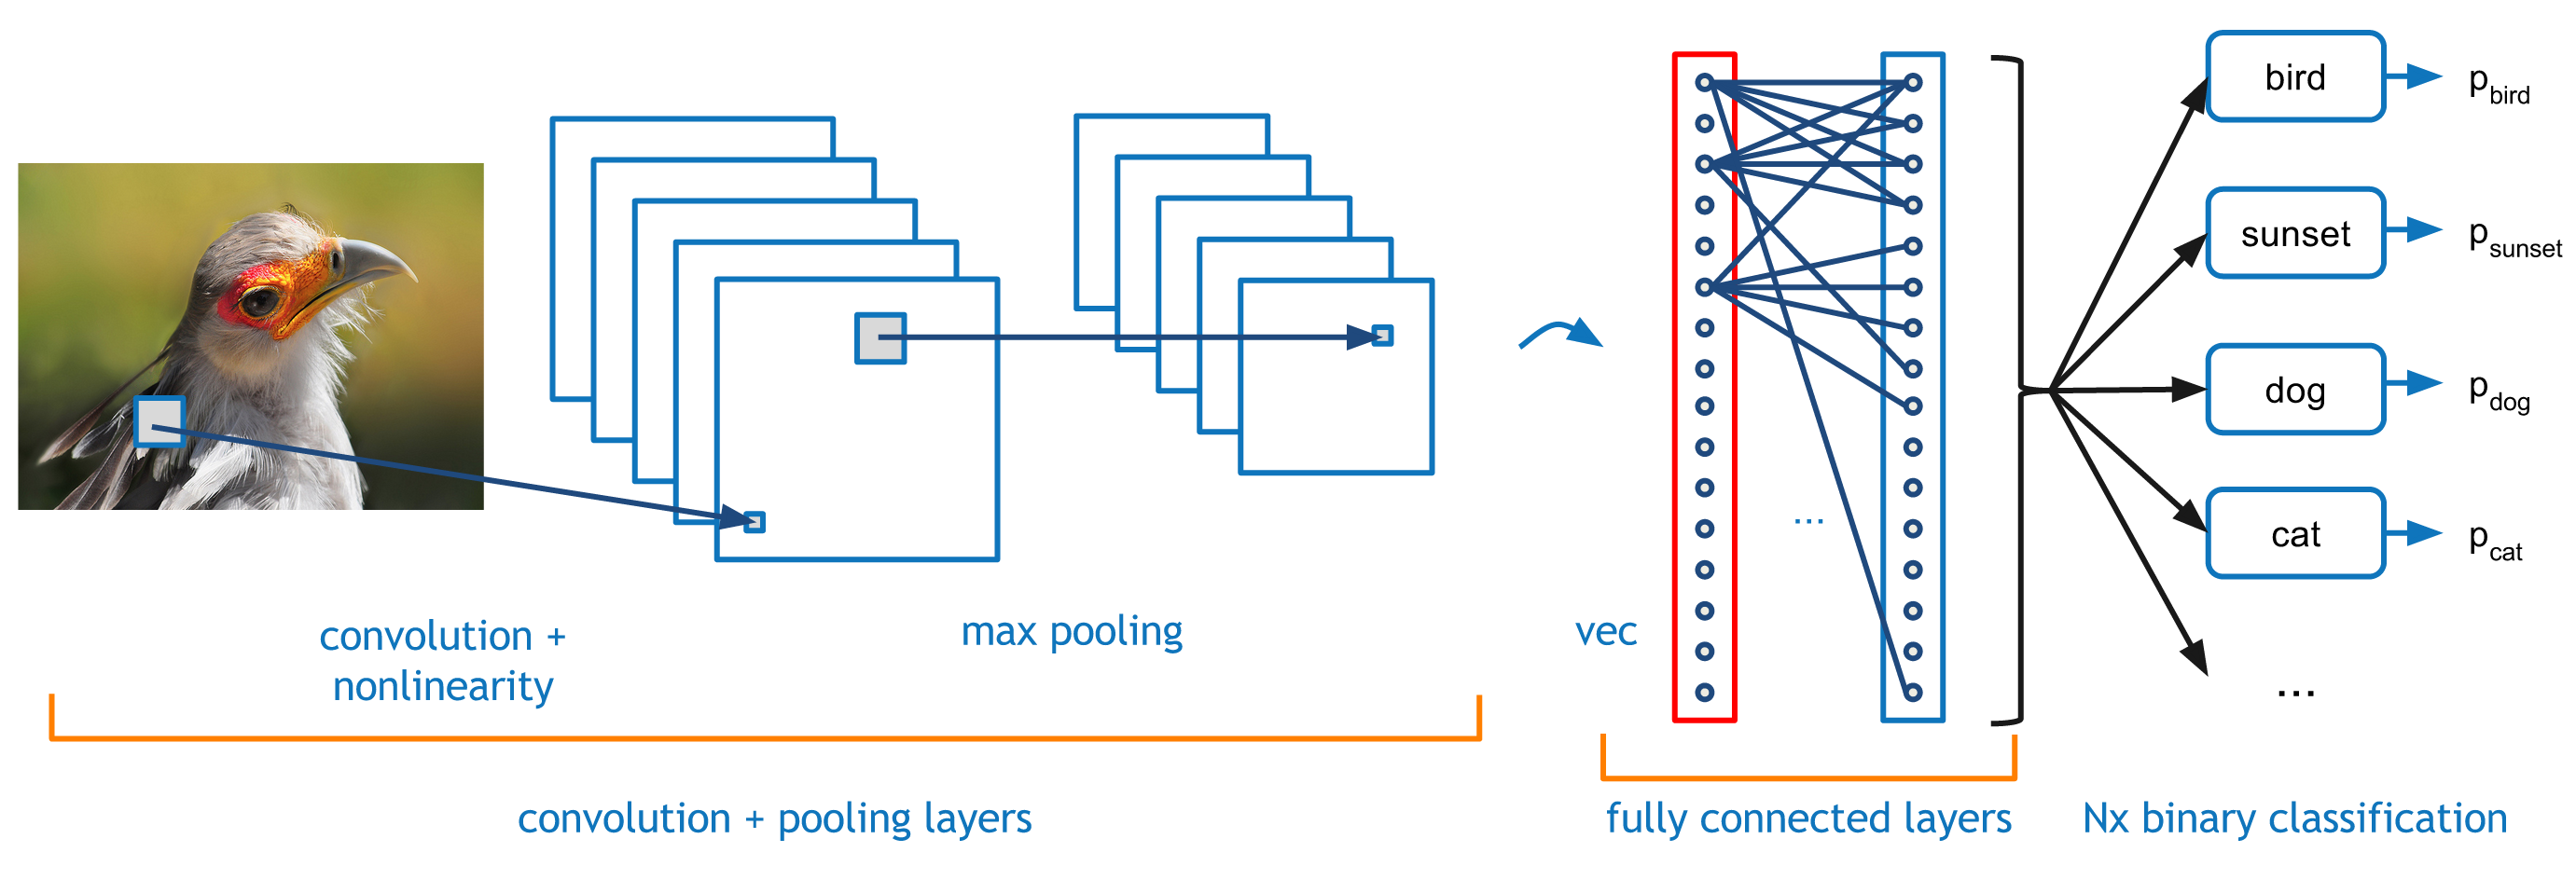
\includegraphics[width=\textwidth]{conv-net2.png}};
        \node[anchor=north west,inner sep=0] at (image.south west) {\url{http://parkorbird.flickr.com/}};
      \end{tikzpicture}

        \textbf{Pooling layer}
        \begin{itemize}
          \item Takes inputs from small region in the feature maps
          \item Reduces resolution and computation in following layers
          \item Increases insensitivity against small shifts
        \end{itemize}

    \end{center}
\end{frame}

\begin{frame}[fragile]
\frametitle{Details: Pooling Layer}
\begin{center}
      \begin{tikzpicture}
      \draw[step=0.5cm,color=gray] (-2,-2) grid (2,2);
      \matrix[matrix of nodes,nodes={inner sep=0pt,text width=.5cm,align=center,minimum height=.5cm, color=gray}]{
      78 & 89 & 29 & 84 & 71 & 33 & 31 & 86 \\
      79 & 27 & 35 & 35 & 94 & 61 & 36 & 19 \\
      22 & 17 & 7 & 45 & 30 & 40 & 29 & 72 \\
      35 & 14 & 11 & 37 & 66 & 76 & 3 & 88 \\
      59 & 4 & 11 & 13 & 22 & 57 & 10 & 52 \\
      62 & 95 & 52 & 19 & 58 & 59 & 22 & 10\\
      9 & 10 & 24 & 42 & 8 & 11 & 87 & 50 \\
      92 & 39 & 53 & 90 & 62 & 78 & 33 & 41\\
       };
       
       \draw[fill=red,opacity=0.4] (-1.0,1.0) rectangle (0.0,0.0);

		\draw[->,-latex',color=red!50!black,line width=0.1cm] (0,0.5) -> (0.9,0.5);
		\draw[->,-latex',color=red!50!black,line width=0.1cm] (-0.5,0) -> (-0.5,-0.9);
		
		\draw[->,>=latex',shorten >=1pt,line width=0.1cm,color=blue!50!black] (-0.5,0.9) to [bend left=50]  node[pos=0.5,midway,above] {$\max p_{ij}$} (-0.75+5.5,0.3);
      \draw[step=0.5cm,color=gray] (-1+5,-1) grid (1+5,1);
      \draw[color=gray] (-1+5,-1) -- (-1+5,1);
		
      \end{tikzpicture}
\end{center}
\vspace{-1em}
\begin{itemize}
\item \textbf{depth} -- number of filters (also known as kernels)
\item \textbf{size} -- dimension of the filter e.g. $2 \times 2$ or $2 \times 2 \times 4$
\item \textbf{stride} -- step size while sliding the filter through the input
\item \textbf{padding} -- behavior of the convolution near the borders
\end{itemize}

\end{frame}

\begin{frame}
  \frametitle{Park or Bird?}
    \begin{center}
      \begin{tikzpicture}
        \node[anchor=north west,inner sep=0] (image) at (0,0) {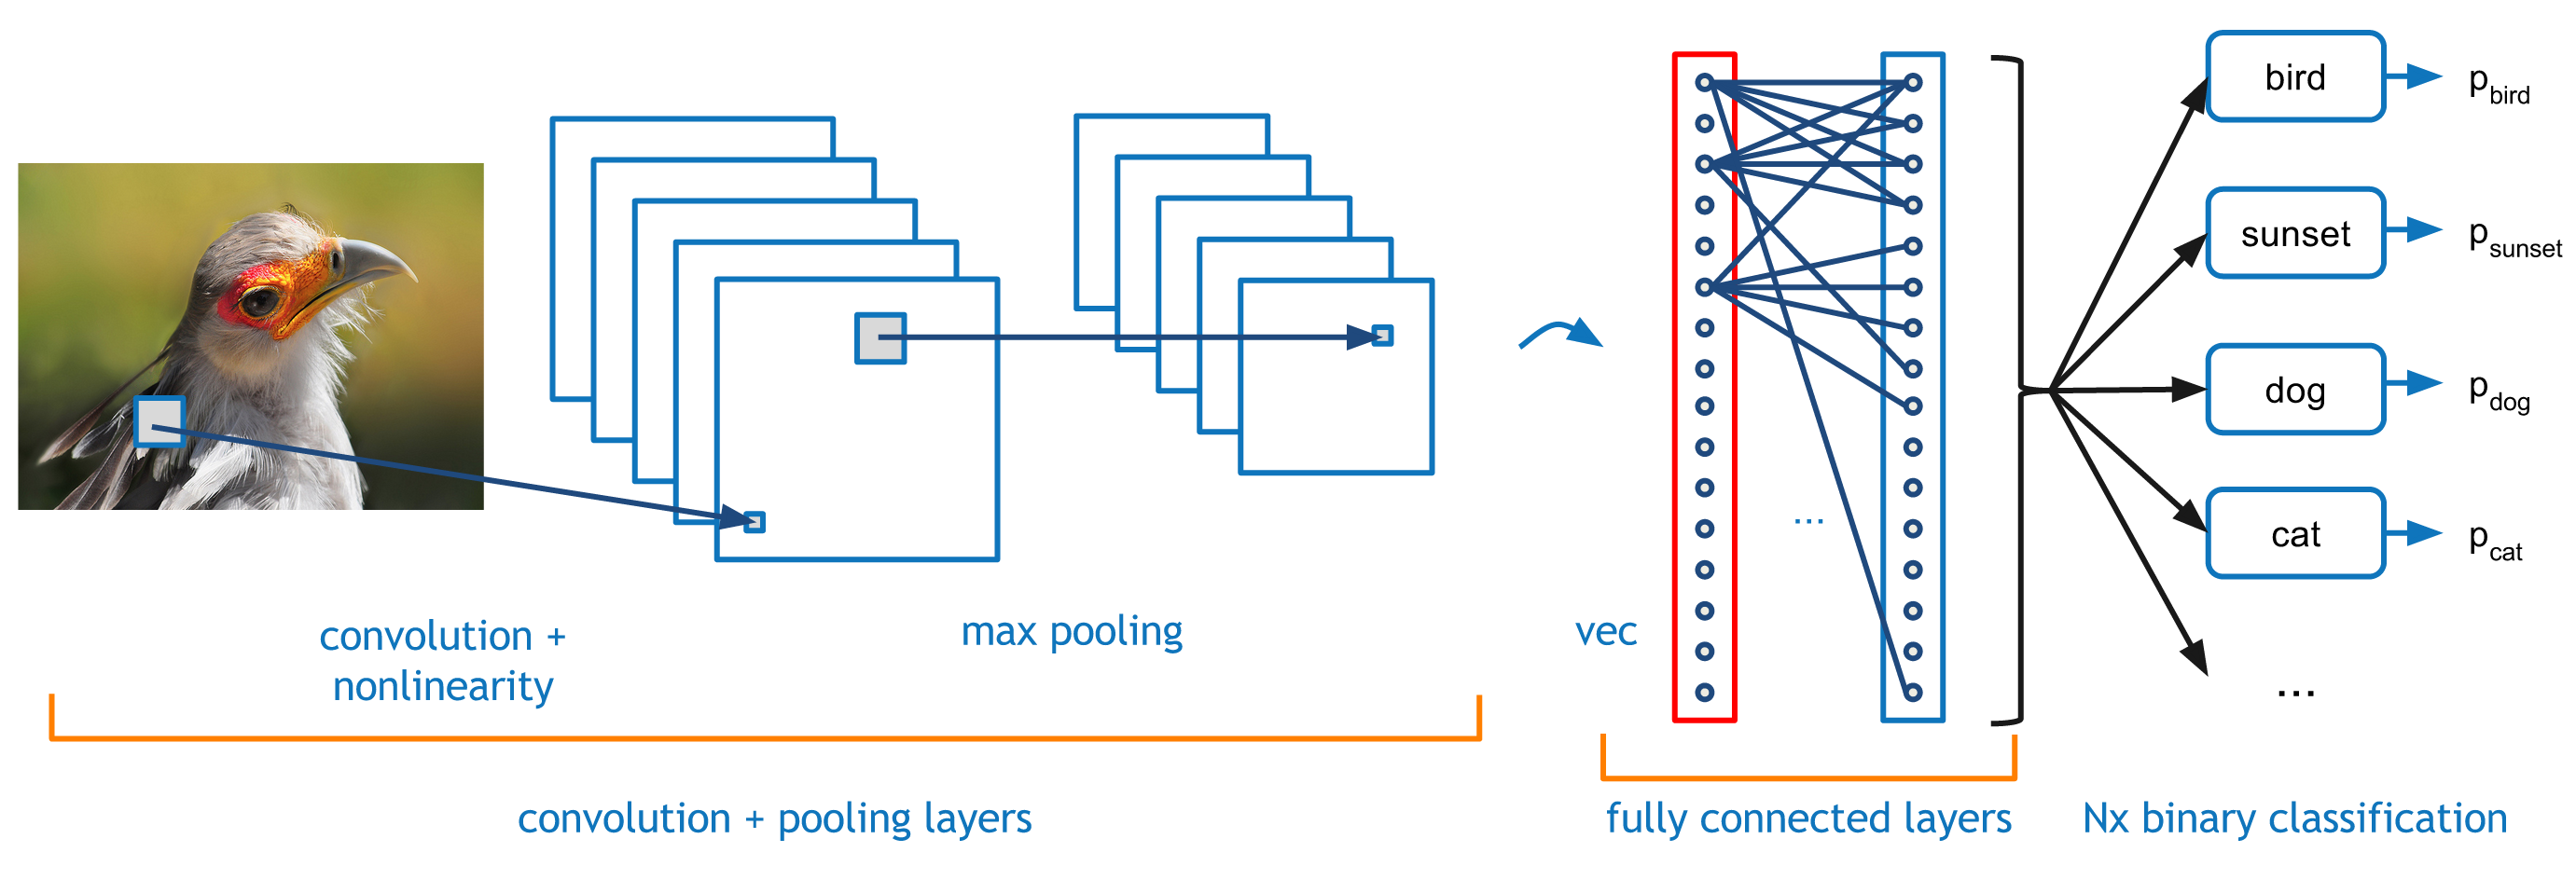
\includegraphics[width=\textwidth]{conv-net2.png}};
        \node[anchor=north west,inner sep=0] at (image.south west) {\url{http://parkorbird.flickr.com/}};
      \end{tikzpicture}

        \textbf{Multiple pairs of convolution and pooling layers}
        \begin{itemize}
          \item Each stage has a larger degree of invariance
          \item Number of features increases as resolution is reduced
          \item Final layer is fully connected with softmax output
        \end{itemize}

    \end{center}
\end{frame}

\begin{frame}
\frametitle{Key Concepts of Representation Learning}

\begin{itemize}
\item \textbf{distributed representations} -- the number of input regions which can be distinguished grows exponentially $\mathcal{O}(2^N)$ in the numbers of parameters $N$; 
\item \textbf{depth} -- the ways to re-use learned features grow exponentially with the depth of the network;
\item \textbf{abstraction} -- the learned features in the deeper layers are increasingly invariant to most local changes of the input;
\item and \textbf{disentangling factors of variation} -- the learned features represent independent properties of the input data.
\end{itemize}

\end{frame}

